\scanpage{112}

\mspage{118}

\uline{Prop 6} Supposons que $f:X\longrightarrow Y$ de $\mathrm{Diag}$ soit \inserted{$\mathbb D$-}propre (resp. $\mathbb D$-lisse). \deleted{Alors $f$ est une $\mathbb D$-fibr. ssi c'est une $\mathbb D$-fibration coh. \deleted{\unsure{fa}} (resp. hom.) faible, ou encore} \inserted{Conditions équivalentes}

a) $f$ est une $\mathbb D$-fib. \unsure{(resp.}

b) $f$ est une $\mathbb D$-fibr. coh. (resp. hom) faible

c) $\forall\,y'\longrightarrow y$ de $Y$, $X_{/y'}\longrightarrow X_{/y}$ (resp. $\,{}_{y\backslash}X_{\deleted{\unsure{y}}}\longrightarrow{}_{y'\backslash}X$) est une $\mathbb D$-équivalence

d) $\forall\,F$ constant sur $Y$, $f_*f^*F$ (resp. $f_!f^*F$) est loc. constant sur $Y$

d') $\forall\,F$ loc constant sur $Y$, $f_*f^*F$ (resp $f_!f^*F$) est loc. constant sur $Y$.

Cela résulte formellement des Prop. 4 et Prop. 5.

\inserted{\uline{Cor.} Supposons $f:X\longrightarrow Y$ Cat-fibrant (resp. Cat-cofibrant). Pour que $f$ soit une $\mathbb D$-fibration, il f. et s. que \deleted{\unsure{les}} pour
% margin note written sideways
tout $u:y\longrightarrow y'$ de $Y$, $u^*:X_{y'}\longrightarrow X_y$ (resp. $u_*:X_y\longrightarrow X_{y'}$) soit une $\mathbb D$-équivalence}

\margin{\figure{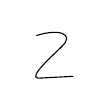
\begin{tikzpicture}[x=0.47cm,y=0.47cm]\draw (0,1.2) .. controls (.6,1.4) and (1.05,1.25) .. (.69,.91) .. controls (.43,.65) and (-.22,.08) .. (.04,.05) -- (1.0,.1);\end{tikzpicture}}}
Il est immédiat que la notion de $\mathbb D$-fibration est stable par chgt. de base, mais il est douteux qu'elle le soit par composition. (Ici encore, \unsure{je pourrais|je devrais|on pourrait} \unsure{ds l'immédiat} faire un contre-exemple, avec $\mathbb D\deleted{\unsure{=k}}=\mathrm{Der}(k\text{-}\mathrm{Mod})$ disons.)

% slanted
\margin{\uline{NB} Si les $\mathbb D$-équivalences sont déjà des Hot-équivalences, alors la notion \unsure{coïncide} avec celle des Hot-fibrations, et elle est stable par composition. \unsure{Égdemt|Égalemt}, si les $\mathbb D$-équivalences sont des $\mathbb D$-équivlc. coh., \unsure{ou} homologiques, alors la notion coïncide resp. avec celle des $\mathbb D$-fibrations cohomologiques (resp. homologiques), ci-dessus. et elle est également stable par \unsure{compos.|composition}}

Autre lacune de la notion : il n'est pas clair, si $f$\inserted{$:X\longrightarrow Y$} est une $\mathbb D$-fibration et $F$ un \deleted{\unsure{$\xi$|$f$}} $\mathbb D$-coeff. sur $Y$, si \deleted{\unsure{$\xi$|$f$}}

\[ f_*f^*F\qquad\text{et}\qquad f_!f^*F \]

se calculent ``fibre par fibre'', comme on attendrait dans le cas d'une ``fibré''.

Par contre, voici un résultat sympa :

% archive sheet number: 112
